\documentclass[a4paper,12pt]{article}
\usepackage{geometry}
\usepackage{fullpage} % Package to use full page
\usepackage{parskip} % Package to tweak paragraph skipping
\usepackage{amsmath}
\usepackage{hyperref}
\usepackage{amsmath,amsfonts,amsthm} % Math packages
\usepackage{graphicx}
\usepackage{listings}
\usepackage{color}
\usepackage{float}
\definecolor{codegreen}{rgb}{0,0.6,0}
\definecolor{codegray}{rgb}{0.5,0.5,0.5}
\definecolor{codepurple}{rgb}{0.58,0,0.82}
\definecolor{backcolour}{rgb}{0.95,0.95,0.92}
\definecolor{brown}{rgb}{0.59, 0.29, 0.0}
\definecolor{beaublue}{rgb}{0.74, 0.83, 0.9}
\definecolor{orange}{rgb}{1.0, 0.5, 0.0}
\definecolor{darkslategray}{rgb}{0.18, 0.31, 0.31}
\def\Xint#1{\mathchoice
	{\XXint\displaystyle\textstyle{#1}}%
	{\XXint\textstyle\scriptstyle{#1}}%
	{\XXint\scriptstyle\scriptscriptstyle{#1}}%
	{\XXint\scriptscriptstyle\scriptscriptstyle{#1}}%
	\!\int}
\def\XXint#1#2#3{{\setbox0=\hbox{$#1{#2#3}{\int}$}
		\vcenter{\hbox{$#2#3$}}\kern-.5\wd0}}
\def\dashint{\Xint-}

% Swap the definition of \abs* and \norm*, so that \abs
% and \norm resizes the size of the brackets, and the 
% starred version does not.
\makeatletter
\let\oldabs\abs
\def\abs{\@ifstar{\oldabs}{\oldabs*}}
%
\let\oldnorm\norm
\def\norm{\@ifstar{\oldnorm}{\oldnorm*}}
\makeatother
\lstdefinestyle{mystyle}{
	backgroundcolor=\color{white},   
	commentstyle=\color{codegreen},
	keywordstyle=\color{blue},
	identifierstyle=\color{brown},
	numberstyle=\tiny\color{codegray},
	stringstyle=\color{orange},
	basicstyle=\footnotesize,
	breakatwhitespace=false,         
	breaklines=true,                 
	captionpos=b,                    
	keepspaces=true,                 
	numbers=left,                    
	numbersep=5pt,                  
	showspaces=false,                
	showstringspaces=false,
	showtabs=false,                  
	tabsize=2
}
\lstset{style=mystyle}

\title{\normalsize AMATH 535: Homework Problem 4.3}
\author{\normalsize Jithin D. George, No. 1622555}
% matrix environment
\newenvironment{mat}{\left[ \begin{array}{ccccccccccccc}}{\end{array}\right]}
\newcommand\bcm{\begin{mat}}
	\newcommand\ecm{\end{mat}}

\begin{document}

\maketitle
	
{\bf 	} 



{\bf Solution:	}
\[N_{t+1}= \frac{R_0^\beta N_t}{[1+ ((R_0-1)/K) N_t]^\beta}\]


At equilibrium, $N_{t+1}=N_t$

We see that $N_t =0$ is a solution.
\[N_{t}= \frac{R_0^\beta N_t}{[1+ ((R_0-1)/K) N_t]^\beta}\]
\[[1+ ((R_0-1)/K) N_t]^\beta=R_0^\beta \]
\[ ((R_0-1)/K) N_t=R_0-1\]
\[N_t^*=K\]

Now, to find the stability, we need the slope.

\[ f' (N_t)= \frac{R_0^\beta+ [(R_0-1)/K] N_tR_0^\beta  - \beta((R_0-1)/K) N_tR_0^\beta  }{[1+ ((R_0-1)/K) N_t]^{\beta+1}}\]
\[ = \frac{R_0^\beta +(1 - \beta)((R_0-1)/K) N_tR_0^\beta  }{[1+ ((R_0-1)/K) N_t]^{\beta+1}} \]

When $N_t^*$ =0,
\[ f' (N_t)= R_0^\beta\]

Since $ f' (N_t) < 1 $ to be stable, the fixed point at 0 is stable for $R_0 < 1$.

For $N_t^*$ =K,
\[ f' (N_t) = \frac{R_0^\beta +(1 - \beta)(R_0-1) R_0^\beta  }{R_0^{\beta+1}}\]

\[ = \frac{1 +(1 - \beta)(R_0-1)  }{R_0}\]
\[ = 1-\beta +\frac{\beta}{R_0}\]

For this to be stable,

\[| 1-\beta +\frac{\beta}{R_0}| <1\]

\[ 1-\beta +\frac{\beta}{R_0} <1 \text{ and } 1-\beta +\frac{\beta}{R_0} >-1\]

\[ \beta >\frac{\beta}{R_0}  \text{ and } \beta -\frac{\beta}{R_0} <2\]
Since both $\beta $ and $R_0$ are known to be greater than 0,
\[ R_0 >1  \text{ and } \beta  <\frac{2}{(1-\frac{1}{R_0})}\]

\[ f' (N_t) = 1-\beta\big(1-\frac{1}{R_0}\big)\]
For a monotonic damping,
\[\beta\big(1-\frac{1}{R_0}\big) <1)\]
\[\beta <\frac{1}{(1-\frac{1}{R_0})}\]

For an oscillatory damping,
\[1<\beta\big(1-\frac{1}{R_0}\big) <2)\]
\[\frac{1}{(1-\frac{1}{R_0})}<\beta <\frac{2}{(1-\frac{1}{R_0})}\]

Here are my plots and python equivalents since my talents in sketching are not so great.
 
\begin{figure}[H] 
	
	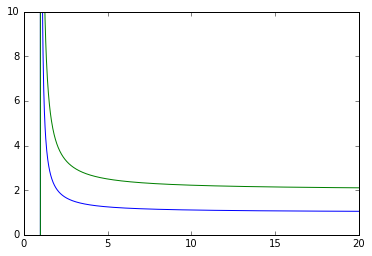
\includegraphics[width=9cm]{curves}
	\caption{Python plots and hand-drawn curves}
\end{figure}

\end{document}